% --- ADJUSTABLE PARAMETERS ---
\def\hsep{4.0}
\def\vsep{1.4}
\def\logicXshift{7.5}
% -----------------------------
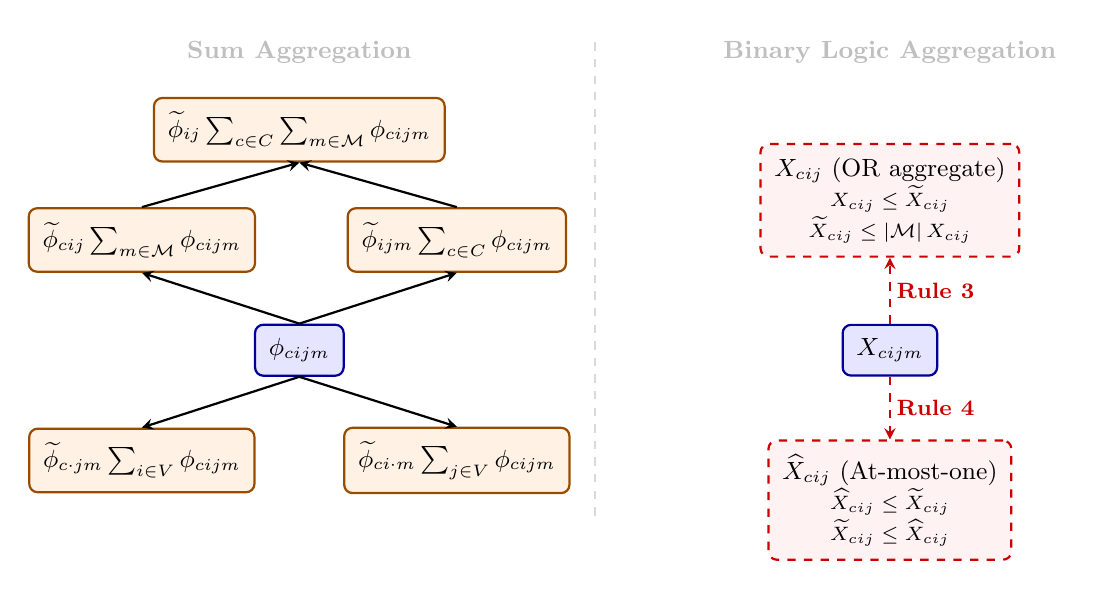
\begin{tikzpicture}[
  every node/.style = {
    draw, rounded corners=3pt, inner sep=5pt,
    align=center, font=\small, thick
  },
  rootBox/.style   = {fill=blue!10, draw=blue!60!black},
  sumBox/.style    = {fill=orange!10, draw=orange!60!black},
  binBox/.style    = {fill=red!5, draw=red!80!black, dashed},
  arr/.style       = {->, >=stealth, thick},
  barr/.style      = {->, >=stealth, thick, dashed, red!80!black},
  lbl/.style       = {draw=none, fill=none, font=\footnotesize\itshape, inner sep=2pt},
  blbl/.style      = {draw=none, fill=none, font=\footnotesize\bfseries, inner sep=2pt, text=red!80!black},
  graylbl/.style   = {draw=none, fill=none, font=\small\bfseries, gray!50}
]

%% --- SUM AGGREGATION SECTION (Left) ---
\node[rootBox] (root) at (0,0) {$\phi_{cijm}$};
\node[sumBox] (Fcij)  at (-\hsep/2, \vsep)
  {$\widetilde{\phi}_{cij} \coloneqq \sum_{m \in \mathcal{M}} \phi_{cijm}$};
\node[sumBox] (Fijm)  at (\hsep/2, \vsep)
  {$\widetilde{\phi}_{ijm} \coloneqq \sum_{c \in C} \phi_{cijm}$};
\node[sumBox] (Fij)   at (0, 2*\vsep)
  {$\widetilde{\phi}_{ij} \coloneqq \sum_{c \in C} \sum_{m \in \mathcal{M}} \phi_{cijm}$};

\draw[arr] (root.north) -- (Fcij.south);
\draw[arr] (root.north) -- (Fijm.south);
\draw[arr] (Fcij.north) -- (Fij.south);
\draw[arr] (Fijm.north) -- (Fij.south);

% Dot notation
\node[sumBox] (dotj) at (-\hsep/2, -\vsep)
  {$\widetilde{\phi}_{c \cdot j m} \coloneqq \sum_{i \in V} \phi_{cijm}$};
\node[sumBox] (doti) at (\hsep/2, -\vsep)
  {$\widetilde{\phi}_{ci \cdot m} \coloneqq \sum_{j \in V} \phi_{cijm}$};

\draw[arr] (root.south) -- (dotj.north);
\draw[arr] (root.south) -- (doti.north);

%% --- BINARY LOGIC AGGREGATION SECTION (Right) ---
\begin{scope}[xshift=\logicXshift cm]
\node[rootBox] (Xroot) at (0, 0) {$X_{cijm}$};
\node[binBox] (XOR)  at (0, \vsep*1.36)
  {$\widecheck{X}_{cij}$ (OR aggregate) \\
   \scriptsize $\widecheck{X}_{cij} \leq \widetilde{X}_{cij}$ \\
   \scriptsize $\widetilde{X}_{cij} \leq |\mathcal{M}|\,\widecheck{X}_{cij}$};
\node[binBox] (XHAT) at (0, -\vsep*1.36)
  {$\widehat{X}_{cij}$ (At-most-one) \\
   \scriptsize $\widehat{X}_{cij} \leq \widetilde{X}_{cij}$ \\
   \scriptsize $\widetilde{X}_{cij} \leq \widehat{X}_{cij}$};

\draw[barr] (Xroot.north) -- (XOR.south)  node[blbl, midway, right] {Rule 3};
\draw[barr] (Xroot.south) -- (XHAT.north) node[blbl, midway, right] {Rule 4};
\end{scope}

%% --- DIVIDER AND LABELS ---
\draw[thick, gray!30, dashed]
  (\logicXshift/2, -1.5*\vsep) -- (\logicXshift/2, 2.8*\vsep);
\node[graylbl] at (0,            2.7*\vsep) {Sum Aggregation};
\node[graylbl] at (\logicXshift, 2.7*\vsep) {Binary Logic Aggregation};

\end{tikzpicture}
